\chapter{Objects' Alignment in Robotics.}  
 \label{chap:opt_rot::intro}
 
 In this chapter, we are concerned with the problem of optimally aligning two vectors, a model point/shape to a ``sensed" or measured point/shape in space \eg $\nu_1, \nu_2 \in \mathbb{R}^n$ to one another with the minimal amount of errors.
 To transform between two pints in the Cartesian coordinate system is akin to the problem of solving a rigid body motion problem where that yields a rotation and a translation. In addition, the scaling factor may be unknown. For translation, there are three degrees of freedom, while rotation has another three viz., the direction of the axis about which we are rotating,  the angle of rotation itself, and the scaling. Three points in either coordinate systems
 give us nine constraints (with each contributing three coordinates), more than enough to find the seven unknowns. IF we discard two of the constraints, we end up with seven equations in seven unknowns that can be developed to allow us to recover the parameters.
 
 There exists many methods of solving this problem. Most of them leverage clever optimization methods and we will be looking into these in this chapter. We could follow the homogeneous transformation scheme we presented in Chapter \ref{chap:intro}, but we would not have an optimal solution. A popular technique in computer geometry and computer vision is to use the iterative closest point algorithm(ICP), an algorithm by Paul Besl and Neil McKay developed out of General Motors Laboratory in the 1990's~\cite{besl1992method}. This is more appropriate for 3D tasks and it describes a generic, representation method for the accurate and computationally efficient registration of three-dimensional (3-D) shapes. The ICP algorithm always converges monotonically to the nearest local minimum of a mean-square distance metric such as an $l_2$ distance, and this convergence rate is of the order of a few iterations. An important property of the ICP algorithm is that it can register data from unfixtured rigid objects with an ideal geometrical model prior to shape inspection. So, if we want to figure out that two geometric representations are congruent, estimate the motion between them in real-time where the correspondences are not known, ICP tends to be really good for such operations.
 
 Now, suppose our dataset is not a complex geometric primitive\footnote{We shall refer to a geometric primitive as a primitive 3D shape such as a cylinder, square, prism and the likes.}, but rather a set of two vectors such that we are tasked with the problem of determining the best \textit{unconstrained transformation} between the two sets of coordinates. We can formulate the problem into a constrained optimization problem and thereafter, through clever factorization, turn the problem into a simple one of factorizing the unconstrained transformation  into a symmetric and orthogonal matrix by which we may solve for the optimal rotation and translation. The algorithm we shall be looking into will be the one that was invented in crystallography in 1976 and updated in 1978 by Wolfgang Kabsch, today dubbed the Kabsch algorithm~\cite{Kabsch1978}. Kabsch showed that a direct solution was possible, irrespective of the non-linear character of the problem.
 
 While other newer algorithms exist, these are the two popular algorithms that we shall be concerning ourselves with in this chapter.
 
 
 \section{Preliminaries}
 \label{chap:opt_rot::prelim}
 
 We will denote the real line by $\mathbb{R}$. An example of a \textbf{metric space} is the \textbf{Euclidean } $n$-\textbf{space} $\mathbb{R}^n$, which consists of $n-$tuples $x = \left(x_1, x_2, \ldots, x_n\right)$ where each $x_i \in \mathbb{R}$. We shall mean an $\mathbb{R}^n$ metric space to have the metric 
 %
 \begin{align}
 d(x,y) = \sqrt{\sum_{i=1}^{n} (y_i - x_i)^2}.
 \end{align} 
 %
 If $n=0$, then $\mathbb{R}^0$ is taken to be a single point $0 \in \mathbb{R}$.
 
 A manifold is ``locally" similar to one of the example metric spaces $\mathbb{R}^n$. Precisely, a \textbf{manifold} is a metric space $\bm{M}$ with the property that, \textit{if $x \in M$., then there is some neighborhood $U$ of x and some integer $n \ge 0$ such that $U$ is homeomorphic\footnote{A homeomorphic mapping means intrinsic topological equivalence between \eg objects. Two objects are homeomorphic if they can be deformed into each other by a continuous, invertible mapping. Such a homeomorphism ignores the space in which surfaces are embedded, so the deformation can be completed in a higher dimensional space than the surface was originally embedded. Mirror images are homeomorphic, as are Möbius strip with an even number of half-twists, and Möbius strip with an odd number of half-twists~\cite{homeomorphic}.} to $\mathbb{R}^n$}. 
 
 A simple example of a manifold is $\mathbb{R}^n$: for each $x \in \mathbb{R}^n$ we can take $U$ to be everything in $\mathbb{R}^n$. 
 
 \begin{quiz}
 	 Suppose we supply $\mathbb{R}^n$ with an equivalent metric, which makes it homeomorphic to $\mathbb{R}^n$, would it also be a manifold?
 \end{quiz}
 
 Another example of a metric space is an open ball in $\mathbb{R}^n$, wherein one can take $U$ to be the entire open ball since an open ball in $\mathbb{R}^n$ is homeomorphic to $\mathbb{R}^n$. Similarly, an open subset $V$ of $\mathbb{R}^n$ is a manifold, \ie for each $x \in V$ we can choose $U$ to be some open ball with $x\in U \subset V$.
 
 
 The \textbf{Euclidean distance} $d(\bm{r}_1, \bm{r}_2)$ between two points $\bm{r}_1 = (x_1, y_1, z_1)$ and $\bm{r}_2 = (x_2, y_2, z_2)$ is given by 
 %
 \begin{align}
 d(\bm{r}_1, \bm{r}_2) = \|\bm{r}_1 - \bm{r}_2\| =\sqrt{(x_2-x_1)^2 + (y_2-y_1)^2 + (z_2-z_1)^2}.
 \end{align}
 
 Suppose that $P$ is a point set with $N_p$ points denoted as $\bm{p}_i: P=\{p_i\}$ for $i=1,\ldots,N_p$. The distance between the point $\bm{q}$ and the point set $P$ is
 %
 \begin{align}
 	d(\bm{q}, P) = \min_{i\in \{1,\ldots,N_p\}}{d(\bm{q}, \bm{p}_i)}.
 \end{align}
 %
 We find that the closest point $\bm{p}_j$ of $P$  satisfies $d(\bm{q}, \bm{p}_j) = d(\bm{q}, P)$.
 
 Suppose that we have a \textbf{line segment} that connects the points, $bm{r}_1, \bm{r}_2$, the distance between the point $\bm{r}$ and the line segment $l$ is
 %
 \begin{align}
 	d(\bm{p}, l) = \min_{x+y=1} \|x\bm{r}_1 + y \bm{r}_2 - \bm{p} \|
 	\label{eq:line_seg}
 \end{align}
 %
 where $x, y \in [0, 1 ]$.
 %
 \begin{homework}
 	Find a closed-form expression for the solution to \eqref{eq:line_seg}.
 \end{homework}
%
Now, if instead of a line segment, suppose we have a set of $N_l$ line segments denoted $l_i$, and let $L=\{l_i\}$ for $i=1,\ldots,N_l$. The \textbf{distance between the point $\bm{p}$ and the line segment set $L$} is 
%
\begin{align}
	d(\bm{p}, L) = \min_{i\in \{1,\ldots, N_l\}} d(\bm{p}, l_i).
\end{align}
%
The closest point $y_j$ on the line segment set $L$ satisfies $d(\bm{p}, y_j) = d(\bm{p}, L)$.
%
Let $g$ be a triangle with the following coordinates  $\bm{r}=(x_1,y_1,z_1), \bm{r}_2 = (x, y, z)$, and $\bm{r}_3 = (x_3,y_3,z_3)$. The \textbf{distance between the point $\bm{p}$ and the triangle $g$} is 
%
\begin{align}
	d(\bm{p}, g) = \min_{x+y+z=1} \| x\bm{r}_1 + y\bm{r}_2 + z \bm{r}_3 - \bm{p} \|
	\label{eq:triangle_dist}
\end{align}
%
where $x \in [0,1], \,\, y\in [0,1],$ and $z \in [0,1]$. 
%
\begin{homework}
	Find a closed-form expression for the problem in \eqref{eq:triangle_dist}.
\end{homework}
 
 Now, if we have a collection of $N_g$ triangles $G$, denoted by $g_i$ such that $G =\{g_i\}$ for $i=1,\ldots,N_g$. The \textbf{distance between the point $\bm{p}$ and the triangle set $G$} is 
 %
 \begin{align}
 	d(\bm{p}, G) = \min_{i\in \{1,\ldots, N_g\}} d(\bm{p}, g_i),
 \end{align}
 %
 and the closest point $y_j$ on the triangle set $G$ satisfies the equality $d(\bm{p}, y_j) = d(\bm{p}, G)$.
 
 \subsection{Distance between a Point and a  Parameterized  Entity}
 %
We define a parametric curve and a parametric surface as single parametric entities $\bm{r}(\bm{u})$, where $\bm{u} = u\in \mathbb{R}^1$ denotes a parameterized curve, and $\bm{u} = (u,v) \in \mathbb{R}^2$ denotes parametric surfaces. We will evaluate a curve within an interval domain \eg $[x,y]$ while the evaluation domain of a surface can be an arbitrarily closely-connected region in a plane. 

We will take the distance from a given point $\bm{p}$ to a parametric entity $E$ to be 
%
\begin{align}
	d(\bm{p}, E)  = \min_{\bm{r}(\bm{u}) \in E} d(\bm{p}, \bm{r}(\bm{u}))
\end{align}
 %
 To compute the point-to-curve and point-to-surface distances, let $F$ be the set of $N_e$ parametric entities denoted by $E_i$, and let $F = \{E_i\}$ for $i = 1, N_e$> The distance between a point $\bm{p}$ and the parametric entity set $F$ is
 %
 \begin{align}
 	d(\bm{p}, F) = \min_{i\in \{1,\ldots, N_e\}} d(\bm{p}, \bm{E}_i).
 \end{align}
 
 To find the distance from a point to a parametric entity, we can create a simplex-based approximation for \eg a line segment or triangle. For a parametric space curve $C =\{\bm{r}(u)\}$, we can compute a polyline $L(C, \delta)$ such that the piecewise-linear approximation never deviates from the space curve by more than a prespecified distance $\delta$. If we tag every point of the polyline with a corresponding $u$ argument values of the parametric curve, we can obtain an estimate of the closest point from the line segment set.
 
 In a similar vein, for a parametric surface $S = \{\bm{r}(u, v)\}$, one can compute a triangle set $G(S, \delta)$ such that the piecewise triangular approximation never deviates from the surface by more than a prespecified distance $\delta$. If we tag each truangle vertex with the corresponding $(u, v)$ argument values of the parametric surface, we can find the $U_a, v_a)$ of the argument values of the closest point from the triangle set. The initial value of $\bm{u}_a$ is assumed to be available such that $\bm{r}(\bm{u}_a)$ is very close to the closest point on the parametric entity.
 
 We can employ a Newtonian minimization approach for solving the point to parametric entity problem when a reliable starting point $\bm{u}_a$ is available. The scalar objective function to be minimized is 
 %
 \begin{align}
 	f(\bm{u}) = \| \bm{r}(\bm{u}) - \bm{p} \|^2.
 \end{align}
 %
 Suppose $\Delta = \left[\partial/\partial \bm{u}\right]^T$ is the vector differential gradient operator, the minimum of $f$ must occur at $\Delta f = 0$. If we have a surface, then we must have $\Delta f = \left[f_u, f_v\right]^T$, with the 2-D Hessian matrix is given by
 %
 \begin{align}
 	\Delta \Delta^T(f) = \begin{bmatrix}
 	f_{uu} & f_{uv} \\
 	f_{uv} & f_{vv}
 	\end{bmatrix}
 \end{align}
 %
 where the partial derivatives of the objective function is
 %
 \begin{subequations}
 	\begin{align}
 	f_u(\bm{u}) &= 2 \bm{r}_u^T(\bm{u})(\bm{r}(\bm{u})-\bm{p}) \\
 	f_v(\bm{u}) &= 2 \bm{r}_v^T(\bm{u})(\bm{r}(\bm{u})-\bm{p}) \\
 	f_{uu}(\bm{u}) &= 2 \bm{r}_{uu}^T(\bm{u})(\bm{r}(\bm{u})-\bm{p}) + 2 \bm{r}_u^T(\bm{u})  \bm{r}_u(\bm{u}) \\
 	f_{vv}(\bm{u}) &= 2 \bm{r}_{vv}^T(\bm{u})(\bm{r}(\bm{u})-\bm{p}) + 2 \bm{r}_v^T(\bm{u})  \bm{r}_v(\bm{u}) \\
 	f_{uv}(\bm{u}) &= 2 \bm{r}_{uv}^T(\bm{u})(\bm{r}(\bm{u})-\bm{p}) + 2 \bm{r}_u^T(\bm{u})  \bm{r}_v(\bm{u}).
 	\end{align}
 \end{subequations}
%
And the update relation for the curve and surface case is
%
\begin{align}
	\bm{u}_{k+1} = \bm{u}_k - \left[\Delta \Delta^T(f)(\bm{u}_k)\right]^{-1} \Delta f(\bm{u}_k)
\end{align}
 %
 where $\bm{u}_0 = \bm{u}_a$. 
  
 \subsection{Distance between a Point and an Implicit Entity}
%
An implicit geometric entity is the zero set of a possibly vector-valued multivariate function $\bm{g}(\bm{r})= 0$. Examples of this distance could be a point-to-curve or point-to-surface distance. The important thing to bear in mind is that the distance metric for an individual entity, once defined, makes the sets of implicit entities straightforward to implement. The distance from a given point $\bm{p}$ to an implicit entity $I$ is given by 
%
\begin{align}
	d(\bm{p}, I) = \min_{\bm{g}(\bm{r}) = 0} d(\bm{p}, \bm{r}) = \min_{\bm{g}(\bm{r}) = 0} \|\bm{r} - \bm{p}\|.	
\end{align}
%
It is helpful to note that when computing the implicit entity distance from a point, the solution is never closed-form and are usually involved. Suppose that $J$ is the set of $N_I$ parametric entities, represented by $I_k$ and $J=\{I_k\}$ for $k=1, N_I$. The distance between a point $\bm{p}$ and the implicit entity set $J$ is given by 
%
\begin{align}
	d(\bm{p}, J) = \min_{k\in \{1,\ldots, N_I\}} d(\bm{p}, \bm{I}_k),
\end{align}
%
and the closest point $\bm{y}_j$ on the implicit entity $I_j$ satisfies the equality $d(\bm{p}, \bm{y}_j) = d(\bm{p}, J)$. In order to compute the distance from a point to an implicit entity, we can create a simplex-based approximation such as line segments or triangles. The point-to-line or point-to-triangle set distance yields an approximate closest point $\bm{r}_a$ which can be used to compute the exact distance.

Typically, we must solve a constrained optimization problem when finding the closest point on an implicit entity, say $\bm{g}(\bm{r})=0$ to a point $\bm{p}$ in order to minimize a quadratic objective function that is subject to a nonlinear constraint 
%
\begin{align}
	\min f(\bm{r}) = \| \bm{r} - \bm{p} \|^2 
\end{align}
%
where $\bm{g}(\bm{r}) = 0$
%
We can form the augmented Lagrange multiplier system of equations to solve the above, \ie 
%
\begin{align}
	\Delta f(\bm{r}) + \bm{\lambda}^T \Delta \bm{g}(\bm{r}) &= 0 \nonumber \\
	\bm{g}(\bm{r}) &= 0
\end{align}
%
where $\Delta - [\partial/\partial \bm{r}]^T$.

\subsection{Quaternions}
The unit quaternion is a four vector $\bm{q}_R = \left[q_0, q_1, q_2, q_3\right]^T$, where $q_0 \ge 0$, and $q_0^2 + q_1^2 + q_2^2 + q_3 = 1$, used to parameterize a rotation matrix. The $3\times3$ rotation matrix generated by a unit rotation quaternion is given by
%
\begin{align}
	R = \bm{q}_R^T \bm{q}_R  = \begin{bmatrix}
	q_0^2 + q_1^2 - q_2^2 - q_3 & 2(q_1q_2 - q_0q_3) & 2\left(q_1q_3 + q_0q_2\right) \\
	%
	2(q_1q_2 + q_0q_3) & q_0^2 + q_1^2 - q_2^2 - q_3 & 2(q_2q_3 - q_0q_1) \\
	%
	2(q_1q_3 + q_0q_2) &  2(q_2q_3 + q_0q_1) & 	q_0^2 + q_3^2 - q_1^2 - q_2 
	\end{bmatrix}
\end{align}
%
For more on unit quaternions, see \autoref{chap:rbd_quat}.

\section{Closed-form Solution using Least Sum of Squares Errors}
\label{chap:opt_rot::least_sum}  
%
As we will see from our sensors, measurements are often inexact, which means we need a way to enforce greater accuracy when determining the transformation parameters. Therefore, we will need more than three points.
%
\begin{figure}[tb!]
	\centering
	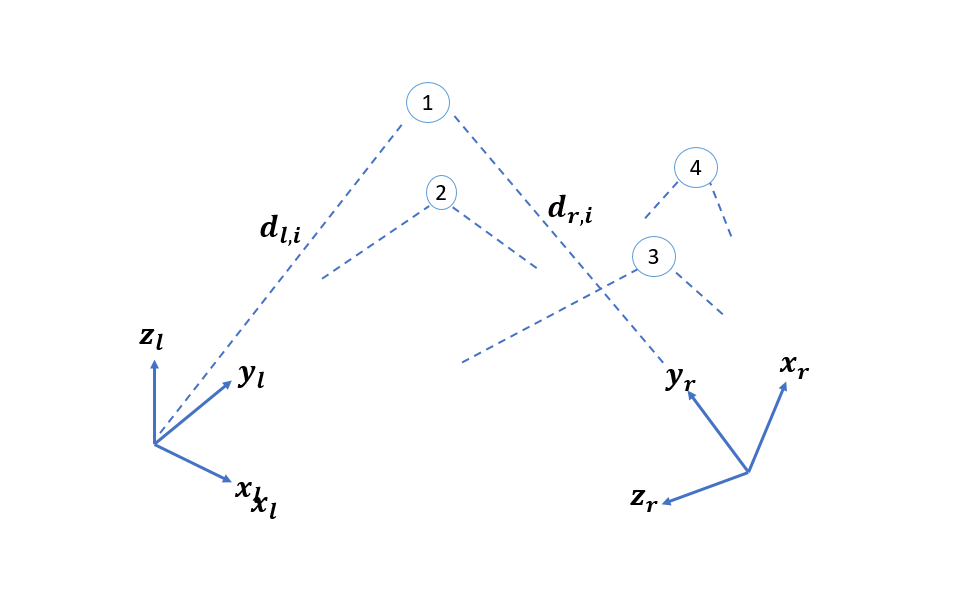
\includegraphics[width=.85\columnwidth]{figures/least_squares.png}
	\caption{Given two coordinate systems, we measure a number of points in the two different coordinate systems. The goal is to find the transformation between the two points.}
	\label{fig:least_squares}
\end{figure}
%
One approach is to minimize the sum of squares of residual errors using various empirical, graphical, and numerical procedures. Because these are iterative in nature, they lead to an approximate solution and while the answer is better, it is imperfect.Iterative methods are repeatedly applied until the residual error is negligible.

There are closed-form solutions which present the absolute orientation in a single step with the best possible transformation given the measurements of the points in the two coordinate systems~\cite{horn1987closed,Kabsch1978}. With these closed-form least sum of squares methods, we do not need to find an initial good guess as is the case for iterative methods.

\subsection{Kabsch Algorithm}
\label{sec:opt_rot::kabsch}
 
 Suppose we have two sets of vectors $\bm{x_n}$ and $\bm{y_n}$ where $n=1,\ldots, N$, and weight $w_n$ that corresponds to each pair $\bm{x_n}$ and $\bm{y_n}$. Our goal is to find an orthogonal matrix $\cup = (u_{ij})$ which minimizes the cost function
 %
 \begin{align}
 	C = \frac{1}{2} \Sigma_n w_n \left(\cup \bm{x_n} - \bm{y_n}\right)^2 
 	\label{eq:kabsch_unconstraint}
 \end{align}
 %
 subject to 
 %
 \begin{align}
 	\sum_k u_{ki} u_{kj} - \delta_{ij} = 0
 	\label{eq:kabsch_constraint}
 \end{align}
 %
 where $\delta_{ij}$ are the elements of a unit matrix. When there is a translation, we can find the centroid of the vector sets to the origin.
 
 In order to solve the problem, we may introduce a symmetric Lagrangian matrix of multipliers, $L = (l_{ij})$ and an auxiliary function as follows
 %
 \begin{align}
 	D = \frac{1}{2} \Sigma_{i,j} l_{ij} \left(\Sigma_k u_{kl} u_{kj} - \delta_{ij}\right)
 \end{align}
 %
 so that we can form the Lagrangian, $E= C+D$. For each condition in \autoref{eq:kabsch_constraint}, we have an independent number $l_{ij}$ so that the constrained minimum of $C$ is part of the free minima of $D$. A free minimum of $D$ can occur if
 %
 \begin{align}
 	\frac{\partial E}{\partial u_{ij}} = \sum_k u_{ik} \left(\Sigma_n w_n x_{nk}x_{nj} + l_{k,j}\right) - \sum_n w_n y_{nl} x_{nj} = 0
 	\label{eq:kabsch_deri1}
 \end{align}
 %
 and 
 %
 \begin{align}
 	\frac{\partial^2 E}{\partial u_{mk} \partial u_{ij}} = \delta_{mi} \left(\Sigma_n w_n x_{nk} x_{nj} + l_{kj}\right)
 	\label{eq:kabsch_deri2}
 \end{align}
 %
 are elements of a positive definite matrix $x_{nk}$ and $y_{nk}$ are the $k$th elements of $\bm{x_n}$ and $\bm{y_n}$. Now, suppose we have a matrix $R=(r_{ij})$ and a symmetric matrix $\bm{S} = \left(s_{ij}\right)$, such that
 %
 \begin{align}
 	r_{ij} = \sum_n w_n y_{ni} x_{nj}
 \end{align}
 %
 and
 %
 \begin{align}
 	s_{ij} = \sum_n w_n x_{ni} x_{nj}.
 \end{align}
 %
 If the matrix \eqref{eq:kabsch_deri2} has $1$ along its diagonal, we must have the minimum of the Lagrangian E to mean that $S+L$ is positive definite, and \eqref{eq:kabsch_deri1} translates to 
 %
 \begin{align}
 U . \left(S+L\right) = R.
 \label{eq:pre_rot}
 \end{align}
 %
 Our goal would be to find a matrix $L$ of Lagrange multipliers so that $\cup$ is orthogonal. We can do this by multiplying both sides of \eqref{eq:pre_rot} by their transposed matrices so that we can get rid of matrix $\cup$ as follows:
 %
 \begin{align}
 	U {(S+L)}^T(S+L) &= {(S+L)}^T{U}^TU(S+L) \nonumber \\
 	&= (S+L)(S+L) = {R}^TR.
 \end{align}
 %
 Now, we know that ${R}^TR$ is a symmetric positive definite matrix so that we can find the eigenvalues $\lambda_k$ and eigenvectors $\bm{v}_k$ using standard procedures \eg single value decomposition. Thus, since $S+L$ is symmetric and positive definite, it must have normalized eigenvectors, $\bm{v}_k$ and positive eigenvalues $\sqrt{\lambda_k}$  so that the Lagrange multipliers are
 %
 \begin{align}
 	l_{ij} = \Sigma_k \sqrt{\lambda_k}; \qquad \qquad \bm{v}_{ki} \bm{v}_{ki} - s_{ij}
 \end{align}
 %
 where $\bm{v}_{ki}$ signifies the $i$th component of $\bm{v}_k$ and the effect of the orthogonal matrix $U$ on these eigenvectors $\bm{a}_k$ is determined from \eqref{eq:pre_rot} which defines the unit vectors $\bm{q}_k$ as 
 %
 \begin{align}
 	\bm{q}_k = U . \bm{v}_k = \frac{1}{\sqrt{\lambda_k}} U (S+L) \bm{v}_k = \frac{1}{\sqrt{\lambda_k}} R \bm{v}_k.
 \end{align}
 
 The solution to find the constraint minimum of the minimum of the proposed cost function in \eqref{eq:kabsch_unconstraint} is then given by,
 %
 \begin{tcolorbox}[title=Kabsch's Optimal Rotation]
 	\begin{align}
 		u_{ij} = \Sigma_k b_{kl} a_{kj}.
 	\end{align}
 \end{tcolorbox}

\subsection{Examples}
%
There are clever ways of solving the optimal rotation between two vectors.

There is a jupyter notebook at the following  link: \href{https://colab.research.google.com/drive/1DL_Hq-Bp-pQuQyR6nDHnzwxIqhj4_Obq}{Kabsch Algorithm and Implementation}. For your convenience, it is included as a pdf file below.

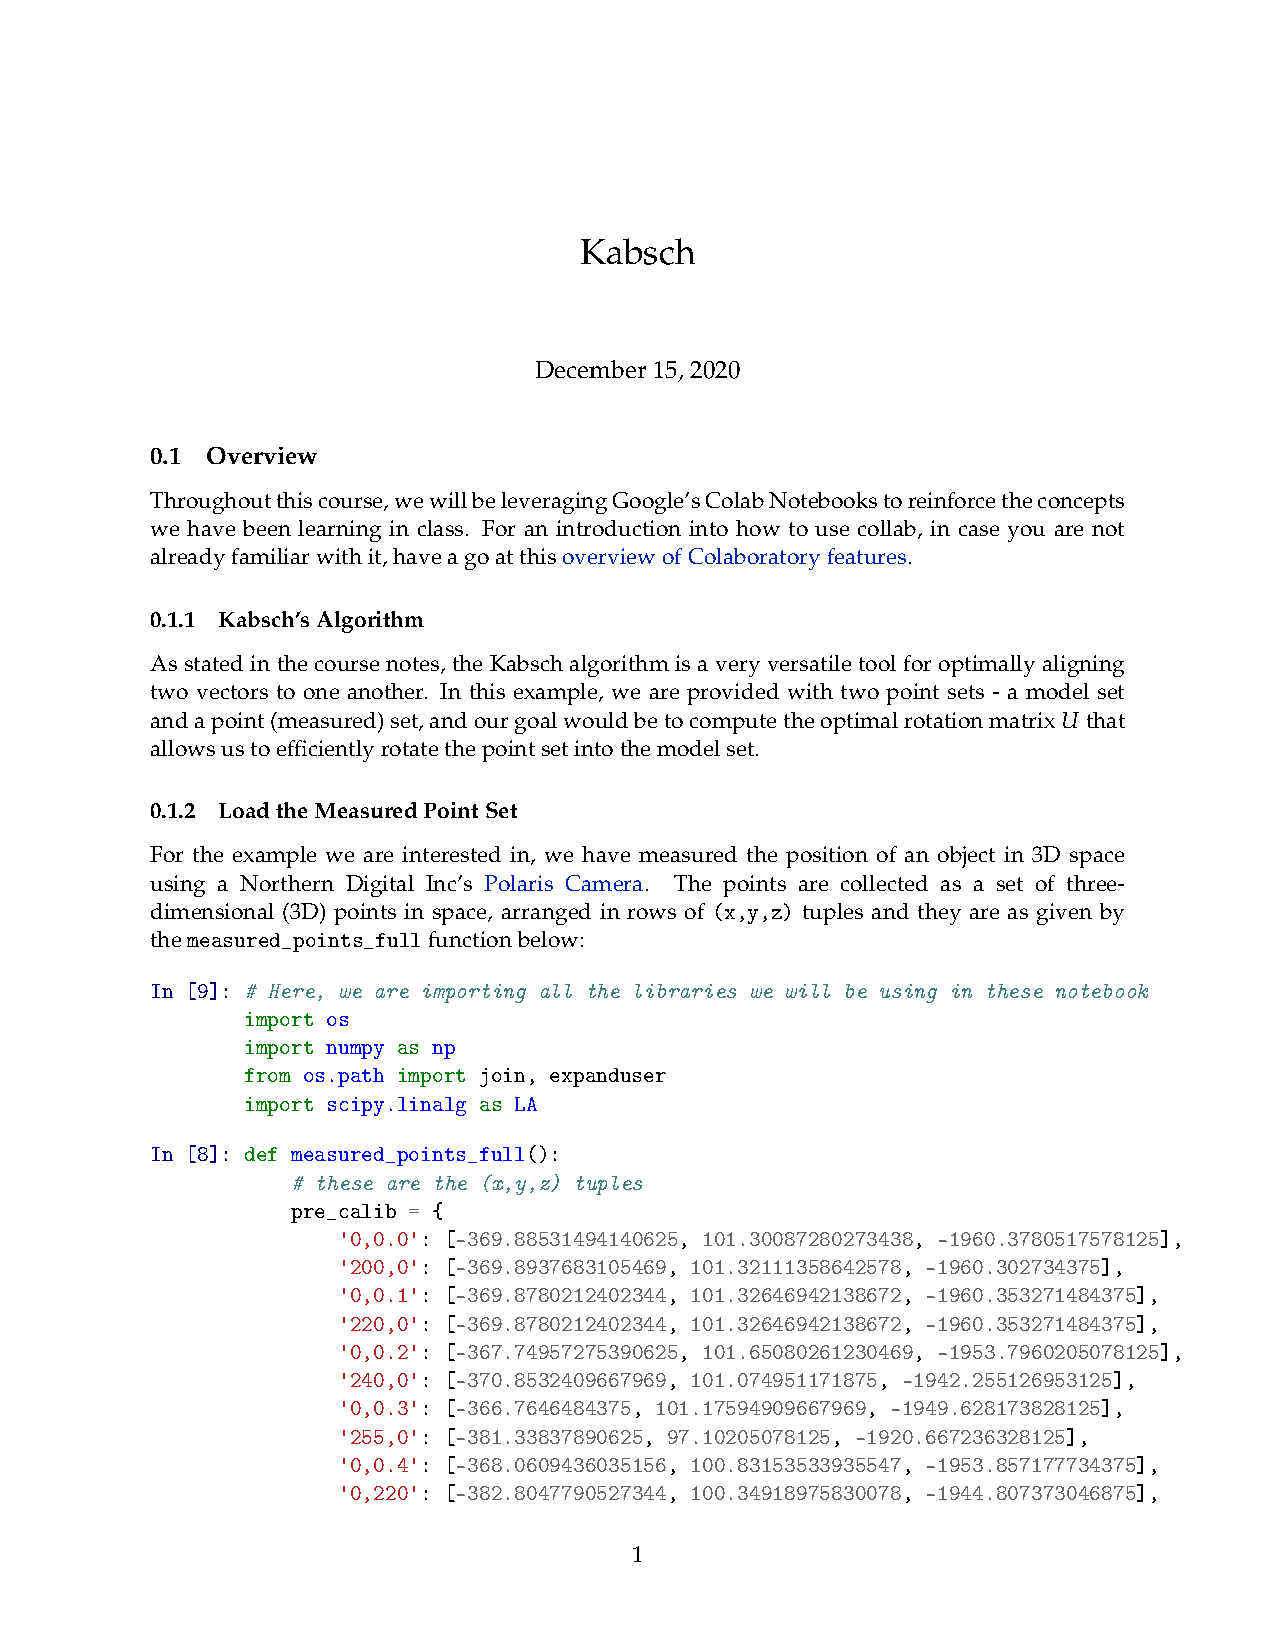
\includepdf[pages=1-]{Kabsch.pdf}

\begin{homework}
	For the following model points $P$ and measured poinyts $Q$, compute the optimal rotation matrices for moving points $Q$ into point $P$. 
	%
	For the three assignments below, report your results within a colab notebook, download the colab notebook as a pdf and upload on Latte.
	\begin{enumerate}
		\item  \begin{align}
			P = \begin{bmatrix}
			-1 & 0 & 0 \\
			%
			0 & 0 & 0 \\
			%
			0 & 1 & 1
			\end{bmatrix},
			%
			\qquad 
			Q = \begin{bmatrix}
			0 & -1 & -1 \\
			0 & -1 & 0 \\
			0 & 0 & 0 \\
			-1 & 0 & 0
			\end{bmatrix}
		\end{align}
		%
		\item \begin{align}
			P = \begin{bmatrix}
			3172.79468418  &  727.52462347  & 7122.70450243 \\
			165.28953155 &  -3552.32467068 & -2045.15346584 \\
			5292.45250241 & -1748.52037006 & -6181.40300009 \\
			1893.07584225  & 5897.19719625  & 3130.41287776
			\end{bmatrix}, 
			\\
			Q = \begin{bmatrix}
			1774.11606309 & -4241.11341178  & 5259.04277742 \\
			6079.70499031  &  -98.14197972 & -3442.0914569 \\
			813.07069876  & 3334.26289147 & -6112.55652513 \\
			1856.72080823 &  2328.86927901  & 6322.16611888 \\
			\end{bmatrix} \nonumber
		\end{align}
		%
		\item For a toy problem, measure the coordinates of an object in the world using your favorite measuring instrument (a 3D camera sensor, iPhone app (e.g. ArkIt), android app e.t.c.). Be sure to record the position of the object at multiple points in world coordinates and make sure that the physical locations of these points are known (these are your model points). Then compute the optimal rotation and translation between the model and measured points.
	\end{enumerate}
\end{homework}

\subsection{Corresponding Point Set Registration with Quaternions}
\label{chap:opt_rot::pt_set_rot}

While the Kabsch algorithm does yield an optimal solution for the rotation of two sets of points that correspond to one another, it leverages the orthonormal rotation matrix with positive determinant in its computations.  This suffers from the non-uniqueness of solutions that arise from reflections. Using matrices straightforward is problematic because we need six nonlinear constraints to guarantee the orthonormality of the rotation matrix. To yield a least squares rotation, and translation, we will generally avoid singular value decomposition (SVD) methods in two and three dimensions since we generally do not want reflections. For $n>3$ in any $n$-dimensional application, the SVD approach, based on the cross-covariance matrix of two point distributions, does generalize easily to $n$ dimensions.

Let $\bm{t} = [t_x, t_y, t_z]^T$ denote the translation vector and $\bm{q}_R = \left[q_0, q_1, q_2, q_3\right]^T$ denote the unit quaternion. Suppose further that the complete registration set of vectors is $\bm{H} = \left[\bm{q}_R | \bm{t}\right]^T$. Now, let $D_l = \{\bm{d}_{l_i}\}$ be the measured set of points which we want to align with the model point set $D_r =\{\bm{d}_{r_i}\}$, where the cardinality, $N_l$ of $D_l$ is same as that of $D_r$, $N_r$, and where each point $\bm{d}_{l_i}$ corresponds to point $\bm{d}_{r_i}$ with the same index. We are looking for a transformation of the form
%
\begin{align}
	D_{r} = a\bm{R}(D_l) + \bm{t}
\end{align}
%
from the left to the right coordinate system as shown in \autoref{fig:2_coords}, where $a$ is a scale factor, and $\bm{t}$ is the translation vector offset. $R(D_l)$ denotes the rotated version of $D_l$. Since we do not expect to have a perfect data, it will be difficult to find a scale factor, a translation and a rotation so that the transformation equation is satisfied for every point. Thus, there will be a residual error, 
%
\begin{align}
	\bm{e}_i = \bm{d}_{r,i} - a \bm{R}(\bm{d}_{l,i}) - \bm{t}
\end{align}
%
and the cost function will minimize the sum of squares is given as, 
%
\begin{align}
f(\bm{s}) = 	\min \| \bm{e}_i\|^2.
\end{align}
%
\subsubsection{Finding Translation}
%
We can find the translation, scale and finally rotation by systematically varying the total error.

Consider the centroids of the measured and point sets,
%
\begin{align}
	\bar{D_l} = \frac{1}{n} \sum_{i=1}^{n} \bm{d}_{l,i}, \qquad 	\bar{D_r} = \frac{1}{n} \sum_{i=1}^{n} \bm{d}_{r,i},
\end{align}
%
so that the new coordinates are 
%
\begin{align}
\bm{d}^\prime_{l,i} = \bm{d}_{l,i} - \bar{\bm{d}}_l, \qquad 	\bm{d}^\prime_{r,i} = \bm{d}_{r,i} - \bar{\bm{d}}_r.
\end{align}
%
If we write $\bm{t}^\prime = \bm{t} - \bar{\bm{t}} + a \bm{R}(\bm{d}_l)$, it follows that we can write the error as 
%
\begin{align}
		\bm{e}_i = \bm{d}^\prime_{r,i} - a \bm{R}(\bm{d}^\prime_{l,i}) - \bm{t}^\prime
		\label{eq:error_w_trans}
\end{align}
%
and the sum of squares of errors becomes
%
\begin{align}
	\sum_{i=1}^{n} \|\bm{d}^\prime_{r,i} - a \bm{R}(\bm{d}^\prime_{l,i}) - \bm{t}^\prime\|^2 \equiv 	\sum_{i=1}^{n} \|\bm{d}^\prime_{r,i} - a \bm{R}(\bm{d}^\prime_{l,i})\|^2 - 2 \bm{t}^\prime . \sum_{i=1}^{n}\left[\bm{d}^\prime_{r,i} - a \bm{R}(\bm{d}^\prime_{l,i})\right] + n \|\bm{t}^\prime \|^2.
\end{align}
% 
The middle term on the right hand side vanishes since the measurements are referred to the centroid and we are left with the first and the third terms. The first term is independent of $\bm{t}^\prime$ and the last term cannot be negative given the squared norm. Thus,  the  total error to be minimized with $\bm{t}^\prime = 0$ is 
%
\begin{tcolorbox}[title=Optimal Translation]
	\begin{align}
	\bm{t} = \bar{\bm{d}}_r - a \,\, R(\bar{\bm{d}}_l)
	\end{align}
\end{tcolorbox}
%
In other words, \textit{the translation is the difference between the right centroid and the scaled and rotated left centroid. }

We can now rewrite the error term from \eqref{eq:error_w_trans} as 
%
\begin{align}
\bm{e}_i = \bm{d}^\prime_{r,i} - a \bm{R}(\bm{d}^\prime_{l,i}) 
\label{eq:error_no_trans}
\end{align}
%
since $\bm{t}^\prime=0$. So the total error to be minimized is 
%
\begin{align}
	\sum_{i=1}^{n} \|\bm{d}^\prime_{r,i} - a \bm{R}(\bm{d}^\prime_{l,i})\|^2.
	\label{eq:resulting_error}
\end{align}


\subsubsection{Finding Scale}
%
Expanding \eqref{eq:resulting_error}, we find that 
%
\begin{align}
	\sum_{i=1}^{n} \|\bm{d}^\prime_{r,i}\|^2 - 2 a \sum_{i=1}^{n} \bm{d}^\prime_{r,i} . R(\bm{d}^\prime_{l,i}) + s^2 	\sum_{i=1}^{n} \|\bm{d}^\prime_{l,i}\|^2,
\end{align}
%
and since rotation preserves distances, $\| R(\bm{d}^\prime_{l,i}) \|^2 = \|\bm{d}^\prime_{l,i}\|^2$, we can write the foregoing as $S_r - 2sD + s^2 S_l$, where $S_r$ and $S_l$ are the sums of the squares of the measurement vectors (relative to their centroids), while $D$ is the sum of the dot products of corresponding coordinates in the right system with the rotated coordinates in the left system. Completing the square in $s$, we find that 
%
\begin{align}
	\left(a \sqrt{S_l} - D/\sqrt{S_l}\right)^2 + \left(S_r S_l - D^2\right)/S_l.
\end{align}
%
If we minimize with respect to scale $a$ when the first term is $0$ or $a = D/S_l$, we find that 
%
\begin{align}
	s = \dfrac{\sum_{i=1}^{n} \bm{d}^\prime_{r,i} \cdot R(\bm{d}^\prime_{l,i})}{\sum_{i=1}^n \|\bm{d}^\prime_{l,i}. \|^2.}
\end{align}

\subsubsection{Finding rotation}
To find the optimal rotation, we note that the cross-covariance matrix $\Sigma_{lr}$ between the sets $D_l$ and $D_r$ is given by 
%
\begin{align}
	\Sigma_{lr} &= \frac{1}{N_l} \sum_{i=1}^{N_l}\left[(\bm{d}_{l,i} - \bar{\bm{d}}_l)(\bm{d}_{r,i} - \bar{\bm{d}}_r)^T\right] \\
	&= \frac{1}{N_l} \sum_{i=1}^{N_l} \left[\bm{d}_{l,i} \bm{d}_{r,i}^T\right] - \bar{\bm{d}}_l \bar{\bm{d}}_r^T.
\end{align}
%
The cyclic components of the skew symmetric matrix $Q_{ij} = \left(\Sigma_{lr} - \Sigma_{lr}^T\right)_{ij}$ are used to construct the column vector $\Delta = \left[Q_{23} \quad Q_{31} \quad Q_{12}\right]^T$, so that the vector is then used to form the symmetric matrix
%
\begin{align}
	Q(\Sigma_{lr}) = \begin{bmatrix}
	\text{tr}(\Sigma_{lr}) & \Delta^T \\
	\Delta & \Sigma_{lr} + \Sigma_{lr}^T - \text{tr}(\Sigma_{lr}) \bm{I}_3
	\end{bmatrix}
\end{align}
%
where $\bm{I}_3$ is the $3\times3$ identity matrix and the unit eigenvector $\bm{q}_R = \left[q_0 \quad q_1 \quad q_2 \quad q_3\right]^T$ that corresponds to the maximum eigenvalue of $	Q(\Sigma_{lr})$ is chosen as the optimal rotation.

\section{Iterative Closest Point}

The Iterative Closest Point (ICP) algorithm applies to the following sets of problems
%
\begin{inparaenum}[(i)]
	\item sets of points,
	%
	\item sets of line segments,
	%
	\item sets of parametric curves,
	%
	\item sets of implicit curves,
	%
	\item sets of triangles,
	%
	\item sets of parametric surfaces, and
	%
	\item sets of implicit surfaces.
\end{inparaenum}
%
To properly describe the algorithm, we choose a data, $P$, which is to be moved or registered/positioned to best align with a ``model" data $X$. It is best if the data and model shape are decomposed into a point set if they are not already in point set form. For triangles and line segments, we use their vertices and endpoints respectively; while for curves and surfaces, an approximation to the vertices and endpoints of triangles and lines are used. Suppose we denote, as before, the number of points in the data shape as $N_p$ and $N_x$ as the number of points, line segments, or triangles in the model shape. The distance metric $d$ between an individual data point $\bm{p}$ and a model shape $X$ will be denoted 
%
\begin{align}
	d(\bm{p}, X) = \min_{\bm{x}(X)} \|\bm{x} - \bm{p} \|.
\end{align}

The closest point in $X$ that yields the minimum distance is denoted $\bm{y}$ such that $d(\bm{p}, \bm{y}) = d(\bm{p}, X)$, where $\bm{y} \in X$.
%
\begin{quiz} 
	%\newline
	\begin{enumerate}
	\item What is the worst case asymptotic computation for the closest point in $X$ and why? %Answer $O(N_x)$
	%
	\item What is the expected worst case computation time?
	\end{enumerate}
\end{quiz}
%
When the closest point computation from $\bm{p}$ to $X$ is performed for each point $P$, that process is worst case $O(N_p, N_x)$. Let $Y$ denote the resulting set of closest points, and $\mathcal{C}$ the closest point operator, \ie 
%
\begin{align}
	Y = \mathcal{C}(P, X).
\end{align}
%
For the resultant corresponding point set $Y$, the least squares registration can be computed as
%
\begin{align}
	content...
\end{align}